\documentclass[letterpaper, 11pt]{report}
\usepackage[utf8]{inputenc}
\usepackage{titlesec}
\usepackage{fullpage} % changes the margin
\usepackage{graphicx} %package to manage images
\graphicspath{ {./images/} }
\usepackage{listings}

\begin{document}
\begin{titlepage}
\vspace*{0.7in}
\begin{center}
\begin{figure}[htb]
\begin{center}

\includegraphics[width=8cm]{univ_logo}
\end{center}
\end{figure}
\vspace*{0.3in}
\begin{Large}
\textbf{SOEN 6011 : SOFTWARE ENGINEERING PROCESSES} \\
\end{Large}
\vspace*{0.1in}
\begin{Large}
\textbf{SUMMER 2021} \\
\end{Large}
\vspace*{0.9in}
\begin{Large}
\textbf{SUPER CALCULATOR} \\
\end{Large}
\vspace*{0.9in}
\begin{Large} 


\textbf{PROBLEM - 4} \\
Error Handling, Debugger and Quality Attributes\\
\end{Large}
\vspace*{0.625in}
\rule{80mm}{0.1mm}\\
\vspace*{0.1in}
\begin{large}
Authors \\
\vspace*{0.1in}
Rokeya Begum Keya\\
\vspace*{0.1in}
Kyle Taylor Lange\\
\vspace*{0.1in}
Sijie Min\\
\vspace*{0.1in}
Manimaran Palani\\ 
\vspace*{0.3in}
\date{\normalsize\today} 
\end{large}
\end{center}
\begin{center}
https://www.overleaf.com/project/610304de4e6b8d24f7c781b6\end{center}
\end{titlepage}
\pagebreak
\section*{\centering{PROBLEM 4 - F2: $tan(x)$}}
\normalsize {SOEN 6011 - Summer 2021} \hfill \textbf{Rokeya Begum Keya} \\
\textbf{ Software Engineering Processes}  \hfill \textbf{40183615} \\
\hfill Repository address : https://github.com/Dakatsu/SOEN6011Calculator
\\\\\\
\section*{Error Handling}
Error handler in a program works when there is any unexpected error condition in a program.
\newline \\
In our Super Calculator, for my function, if there is any input without integer(degree), the program will notify the user by sending an error massage. 
\newline\\
numericInputCheck(inputDataString)  will provide an error massage of type NumberFormatException when the input will not be an valid number.
\newline\\
In our supper Calculator the error handling is done by try..catch method.

\section*{Debugger}
   \section*{Description:}
In this project I used the Eclipse debugger. When I run my program in Eclipse, it automatically open my program with debug form. In Eclipse debugging, It allows the function to run the code step by step and detect the debug.  \\

\textbf{Advantages}
\begin{itemize}
\item In eclipse debugger, there is auto-completion which makes it easy to use.
\item In eclipse debugging mode, function's variable can be changed.
\item It provides Breakpoints which increase the efficiency of debugging.  
\item By using eclipse debugger, one can debug not only in java but also in many other languages.
\end{itemize}

\textbf{Disadvantages}
\begin{itemize}
\item Some programs have multi-threading, which makes it more complicated to control the program.
\item If there is any time limitations in a function,it will increase the difficulty level of debugging in eclipse.
\end{itemize}
\newpage
\section*{Quality Attributes}
\begin{itemize}
  \item \textbf{Correctness:} For my tangent $tan(x)$ function, I had to test different positive and negative integer values (degree) to compare the accuracy with a scientific calculator. Overall, the value of my function and the scientific calculator are nearly similar.
  \item \textbf{Efficiency:} As it is a super calculator, many repetitions of mathematical equations increase the program execution time. As I did not use any complex function structure, it does not show any complexity and can compile quickly.
  \item \textbf{Maintainability:} I try to make it easy to understand and maintain the code easily by giving some comments before every function's beginning and providing the ending comments and I also added javadoc comments to increase the maintainability. 
  \item \textbf{Robustness:} I apply different wrong inputs to see how my program can handle the error; it can give the user an error message when there is any incorrect input.
  \item \textbf{Usability:} I give a common name of my function so that the other users can easily understand the function. 
  \end{itemize}
  
\section*{Checkstyle} checkstyle- plug-in for Eclipse is used to check the quality of my source code. checkstyle is mainly used to improve the formation of the code. It is a simple process to install the checkstyle in Eclipse. It has Sun and Google-style support, and I choose the Google-style support. It can automatically generate the issues of the code. I have made some changes after checking the quality of my code using checkstyle. However, after getting my code review from my team member, I added the Javadoc comments to my code function, which makes my code easy to understand.
\begin{itemize}
\item \textbf{Advantage:} checkstyle is mainly used to improve the formation of the code. It is a simple process to install the checkstyle in Eclipse.It can automatically generate the issues of the code.
\item \textbf{Disadvantage:} There is less space between the 'error,' 'warnings'  and 'description,' 'resource' and 'path,' less space, making it challenging to understand the problem correctly.
\end{itemize}
\pagebreak

\section*{\centering{PROBLEM 4 - F3: Hyperbolic Sine, $sinh(x)$}}
\normalsize {SOEN 6011 - Summer 2021} \hfill \textbf{Kyle Taylor Lange} \\
\textbf{ Software Engineering Processes}  \hfill \textbf{27627696} \\
\hfill Repository address : https://github.com/Dakatsu/SOEN6011Calculator

\section*{Implementation Difficulties}
\normalsize{There were two main difficulties to making the function implementation efficient and accurate. \\\\
The first issue was that the run-time of the Greatest Common Denominator and Root functions. The runtime of the GCD function is roughly proportional to the size of the input integers, and the possible gains from reducing the size of the rational numbers were often offset by the time spent trying to find a GCD. The root function also tended to increase in computation time when the root level increased. \\\\
The second issue was the limitation of the double type, which uses a binary floating point. While testing showed that the result of the function with integer inputs was accurate to the built-in Java $Math.sinh(x)$ function to at least 12 digits, the accuracy of decimal numbers varied in part due to the multiplication of the integral result by the decimal portion. Doubles also have a maximum size, meaning that raising $e$ to above $\pm$709 resulted in a $\pm$ $Infinity$ value being returned. An attempt at coding a new type that could handle math on large decimal numbers with no floating point error and arbitrary precision was done poorly and ultimately scrapped, so $\pm$ $e^(709)$ remained the cap for values of the integral and numerator portion of the rationalized decimal. \\\\
The above two issues resulted in calculations beyond $\pm$ 709 returning $\pm$ $Infinity$ as is standard for doubles, and a drastic decrease to accuracy in numbers with decimals that do not simplify into fractions with small integers or are simply too large to quickly find the GCD.}

\section*{Code Qualities}
\normalize{Despite the aforementioned issues with decimal values, the calculations for integral values are very correct. Both unit testing and manual testing verified the correctness of those values. Manual testing and debugging also ensured that the calculations are done quickly. In regards to maintainability, the function code is fully commented with detailed Javadoc comments, and the subordinate functions are separate to allow re-use and modularity. Magic numbers are declared as constants, allowing them to be modified in future revisions of the program. All functions are implemented within one static library/utility class, making them directly callable instead of requiring an object to be instantiated.}

\section*{Error Handling}
\normalsize{The $sinh$ function itself handles issues with the format of the input. It takes a $String$ as input to allow multiple number formats and improve accuracy over binary floating point inputs, and it will throw $NumberFormatException$ classes when it receives unparsable input.}

\section*{Debugging and Checkstyle}
\normalize{The stock Eclipse debugger was used to test the function. Adding breakpoints helped trace program flow and uncover the causes of program stalls and where values differed from the expectations of the programmer. There were no notable disadvantages to using this built-in debugger over the one built into IntelliJ. \\\\
The Checkstyle tool was used to check the formatting of the source code. It was easy to install and use due to it being available as a plug-in for the Eclipse IDE and coming with both Sun/Oracle and Google style support. Running Checkstyle revealed that the code mostly conformed to its guidelines, but it nonetheless uncovered a few inconsistencies. Most parameters and constants were subsequently changed to be final since they are not modified in the function body, lines were split to not exceed too many characters, and an else statement was moved to the same line as the preceding bracket. The class was also given an empty private constructor to ensure it could never be instantiated due to it being a static utility/library class. The only two noticeable annoyances were the inconsistencies in style being labelled as \textit{errors} instead of \textit{warnings}, and that the way the lines with these \textit{errors} were highlighted by Eclipse and/or Checkstyle made it difficult to find issues like an extra space.}

\pagebreak

\section*{\centering{PROBLEM 4 - F5}}
\normalsize {SOEN 6011 - Summer 2021} \hfill \textbf{Sijie Min} \\
\textbf{ Software Engineering Processes}  \hfill \textbf{40152234} \\
\hfill Repository address : https://github.com/Dakatsu/SOEN6011Calculator
\\\\\\\\\\


 \section*{{Error Handling}}
\\The regular handling mechanism allows the program to deal with the exception in accordance with the pre-set exception handling logic of the code when an exception occurs, so that the program can return to normal and continue execution as much as possible, and keep the code clear.
\\For function 5, the constant b cannot be negative, and for the ln(x) function, x should be greater than 0. When the input of the function is out of the allowable range, the function will throw an exception, and the exception message is "math range error". When using function 5, you need to use try...catch... to handle the exception.
\section*{{Debugger}}
\\Used Eclipse to write and debug code. Eclipse's built-in debugger provides a convenient means of debugging. You can find bugs by debugging with breakpoints and monitoring variables. It can also viewed the method call relationship and the thread method call stack.
 \begin{figure}[htp]
    \centering
    \includegraphics[width=16cm]{F5p4}
    \caption{The check style of F5}
    \label{fig:galaxy}
\end{figure}
 \begin{center} 


 
 
 
 
 \end{center}
  \begin{thebibliography}{}
 
\bibitem{test1}
Mike Spivey. "The fuzz Manual" Manual and software copyright .J. M. Spivey 1988, 1992, 2000


\end{thebibliography}   
 
 
 
\pagebreak

\section*{\centering{PROBLEM 4 - F7 : \(x^y\)}}
\normalsize {SOEN 6011 - Summer 2021} \hfill \textbf{Manimaran Palani} \\
\textbf{ Software Engineering Processes}  \hfill \textbf{40167543} \\
\hfill Repository address : https://github.com/Dakatsu/SOEN6011Calculator
\\
\section*{\textbf{Problem 4 - Description}}
This section presents an overview of the source code of the Super Calculator application \\(F7-Power Function)  and the
practices followed during the development.
\vspace{0.4cm}
\section*{Error Handling}
When an exception occurs in Super Calculator, Its considered that the exception is "thrown."
\newline\\
numericInputCheck(inputDataString)  throws an exception of type NumberFormatException when the value entered in the text field is any character other than real numbers. \newline\\
When an exception is thrown, it is possible to "catch" the exception and prevent it from crashing the program. This is done with a try..catch statement in the super calculator. 
\newline\\\\
In simplified form, the syntax for a try..catch statement can be:
\\
\begin{lstlisting}
try {
   statements-1
   ...
   numericInputCheck(inputDataString)
   ...
}
catch ( NumberFormatException exception) {
   statements-2
}
\end{lstlisting}
\begin{figure}
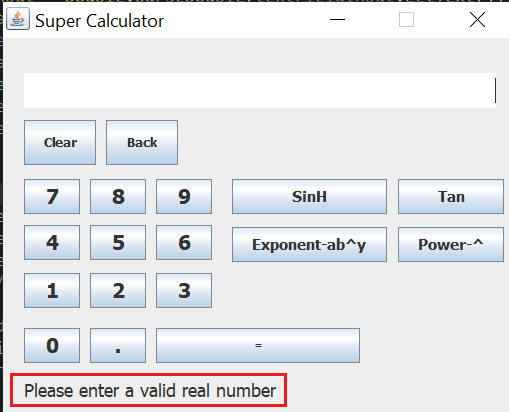
\includegraphics[width=0.6\textwidth]{error_handling_F7}
\centering
\caption{ An Error message in the Super Calculator that displays if the input is not accepted.
}
\end{figure}
\newpage
\section*{Debugger}
Eclipse has a standard debugger which allows the program to open in debug mode.It supports both step by step debugging and break point based debugging.It offers, breakpoints , checkpoints and multiple views which enhance the experience of debugging.\\

\textbf{Advantages}

\begin{enumerate}
  \item Can add any variable that one want to monitor to watch list.\
  \item Eclipse debugger allows to remote debug a process on any other machine .\
  \item One can move the current execution while executing . \
  \item One can step in and out of the code base based on whether it matters or not.\
  \item The debug perspective offers additional views that can be used to troubleshoot an application like Breakpoints, Variables, Debug, Console etc. \
  \item The Eclipse Debugging Platform helps developers debug by providing buttons in the toolbar and key binding shortcuts to control program execution. \
\end{enumerate}

\textbf{Disadvantages}
\begin{enumerate}
\item Debugging with eclipse will become difficult when the execution  of a particular function is time bound or if there is usage of sleep statements inside the program. \
\item It is difficult to monitor the programs that uses mutli threading . \
\end{enumerate}
\newpage
\section*{Quality Attributes}
Quality attributes assessed while implementing the algorithm  are :\\
\begin{itemize}
  \item \textbf{Correctness:} Since I used taylor series for approximating the power function , I had to test with different number of iterations ranging from 10 to 100 to come to a conclusion on the optimum number of iterations to ensure the correctness of the function.Based on my tests , I came to a conclusion that to have minimum difference between expected output and actual output , the number of iterations needed is 13.
  \item \textbf{Efficiency:} As number of iterations increase, it increases the time of execution of the program but less no of iterations have a big impact on the correctness of the program.Hence to have a above average efficiency and a decent correctness I have chosen the no of iterations as 13.
  \item \textbf{Maintainability:} I have refactored the code and included the comments to improve the maintainability and understand-ability of the code.Have a test file to ensure that any changes made doesn't have an effect on the existing functionality of the program.
  \item \textbf{Robustness:} I have handled the situation where the user might give a wrong input such as a string in the place of a double .Hence the program doesn't crash and notifies the user with an appropriate error message.This increases the robustness of the program.
  \item \textbf{Usability:} I am packaging my program in an executable jar file so that other users can use my file without any difficulties.This increases the usability of the program.
\end{itemize}
\vspace{0.4cm}
\section*{Code Quality Check}
To check the quality of the Super Calculator's source code, Checkstyle tool is used. This section presents an overview of Checkstyle tool.
\begin{itemize}
    \item Checkstyle is a development tool to help programmers write Java code that adheres to a coding standard.
    \item It automates the process of checking Java code to spare humans of this boring (but important) task.
    \item This makes it ideal for projects that want to enforce a coding standard.
    \item Checkstyle is highly configurable and can be made to support almost any coding standard.
\end{itemize}
\begin{figure}
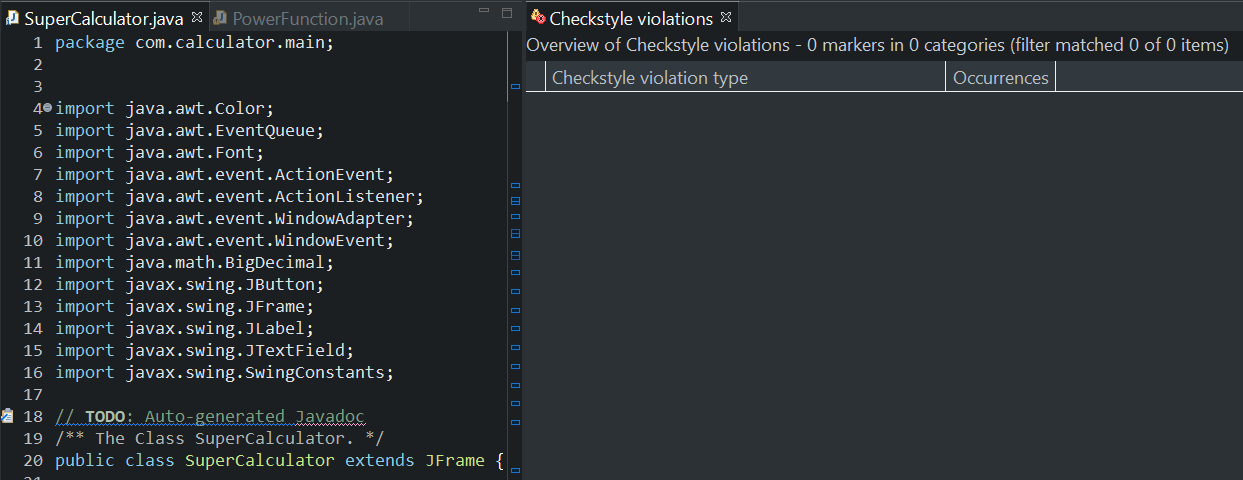
\includegraphics[width=1\textwidth]{Super_Calculator_Checkstyle}
\centering
\caption{ \textbf{Overview of CheckStyle Violations} - SuperCalculator.java - \textbf{0 Violations}.
}
\end{figure}
\begin{figure}
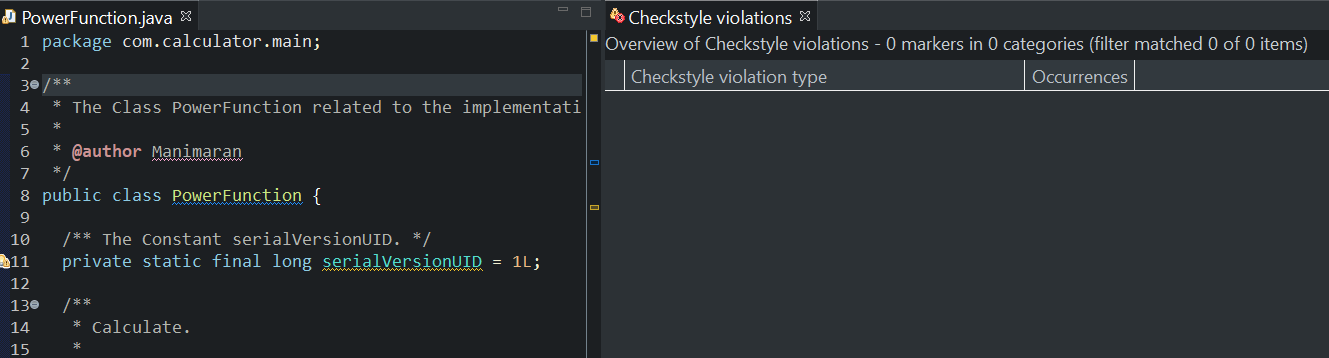
\includegraphics[width=1\textwidth]{Power_Function_Checkstyle}
\centering
\caption{ \textbf{Overview of CheckStyle Violations} - PowerFunction.java - \textbf{0 Violations}.
}
\end{figure}
\begin{figure}
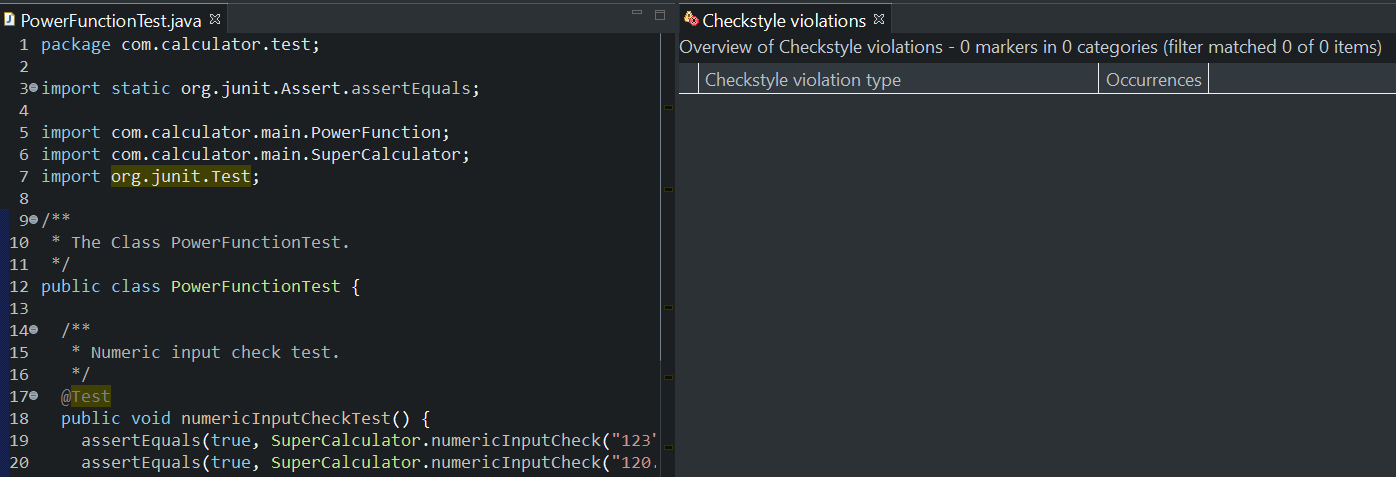
\includegraphics[width=1\textwidth]{Power_Function_TestCases_Checkstyle}
\centering
\caption{ \textbf{Overview of CheckStyle Violations} - PowerFunctionTest.java - \textbf{0 Violations}.
}
\end{figure}
\newpage


\end{document}
